\section{Μοριακά Νέφη και διαγαλαξιακός χώρος}
Στον μεσοαστρικό χώρο υπάρχει μια τεράστια ποσότητα ύλης υπό τη μορφή αερίου και σκόνης. Η ύλη αυτή, που μπορούμε να πούμε ότι είναι το πρωτόγεννες καύσιμο στη διαδικασία αστρικής δημιουργίας των γαλαξιών, αποτελείται περίπου κατά 99\% από αέριο και κατά 1\% από σκόνη με τη συνολική της μάζα για το δικό μας γαλαξία να είναι της τάξης των \SI{1e9}{ M_{\odot}}, ενώ η πυκνότητα της κυμαίνεται από \SIrange{1e-4}{1e6}{cm^{-3}}.

\begin{marginfigure}
	\label{fig:21}
	\centering
	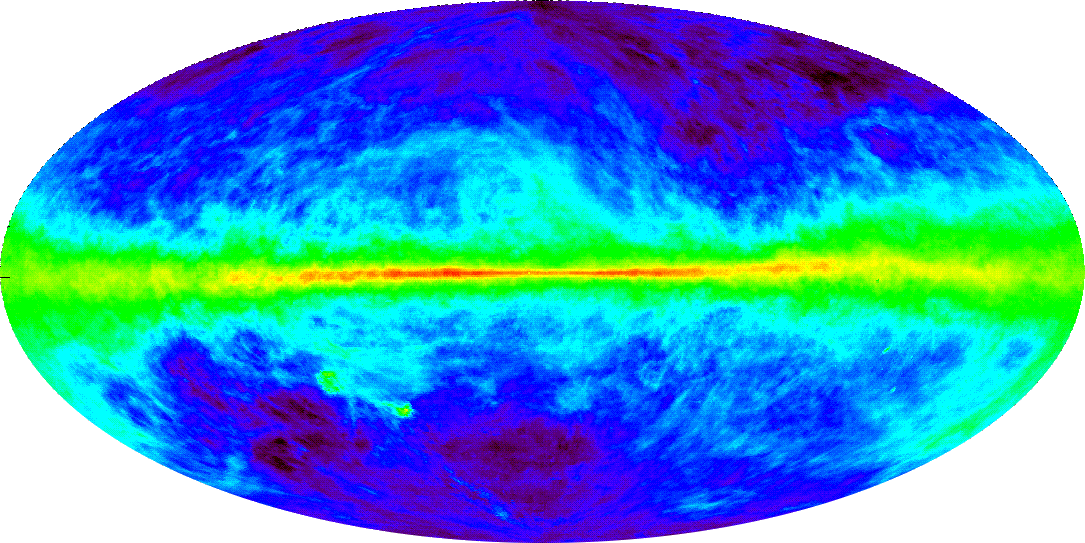
\includegraphics[width=1\linewidth]{Images/21.png}
	\caption{Εκπομπή του \ce{HI} στα 21.1 cm (Kalberla et al., 2005)%\cite{kalberla_2005}.
		H εκπομπή της γραμμής \SI{21}{cm} στα ραδιοκύματα που οφείλεται στη μετάπτωση αντιστροφής του spin του πρωτονίου και του ηλεκτρονίου στη βασική κατάσταση του ατόμου του Υδρογόνου. Η ενεργειακή διαφορά των καταστάσεων είναι 
		$h \nu=\SI{6e-6}{eV}$, η οποία αντιστοιχεί σε μήκος κύματος \SI{21}{cm}.}
\end{marginfigure}

\begin{marginfigure}
	\label{fig:Ha}
	\centering
	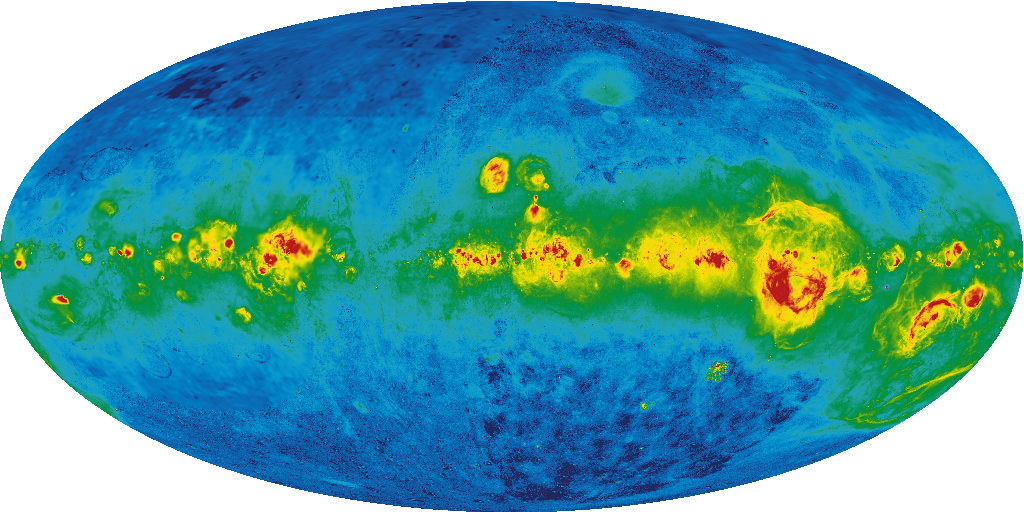
\includegraphics[width=1\linewidth]{Images/Ha.png}
	\caption{Εκπομπή Ha από συνδυασμό τριών διαφορετικών παρατηρήσεων (WHAM - VTSS - SHASSA) \cite{finkbeiner_2003}. Η εκπομπή Ha (\SI{656.28}{nm}) προέρχεται από την επανασύνδεση ιονισμένων ατόμων υδρογόνου κοντά σε θερμούς αστέρες O και B (\ce{HII} Regions).}
\end{marginfigure}


\paragraph{Μεσοαστρικό Αέριο} 
Το Μεσοαστρικό Αέριο παρατηρείται σε νεφελώδη μορφή και αποτελείται κυρίως (περίπου το 90\%) από υδρογόνο σε ατομική \ce{(H)}, ιονισμένη \ce{(HII)} και μοριακή \ce{(H2)} κατάσταση. Δεύτερο σε αναλογία είναι το Ήλιο \ce{(He)} (περίπου 9\%) ενώ το υπόλοιπο 1\% είναι βαρύτερα στοιχεία (\ce{C},\ce{O},\ce{Ne},\ce{Mg},\ce{Fe}, κ.α.) και μόρια (\ce{CO},\ce{CS}, κ.α.).


\paragraph{Μεσοαστρική Σκόνη}
%\begin{figure}[h]
%	\centering
%	\includegraphics[width=\medpage]{images/dust_emission_planck.png}
%	\caption{Εκπομπή της σκόνης του Γαλαξία μας όπως τη χαρτογράφησε το Planck.\cite{planck_2014}}
%\end{figure}

Η Μεσοαστρική Σκόνη αποτελείται κυρίως από άνθρακα και πυρίτιο σε ενώσεις με Υδρογόνο, Οξυγόνο, Μαγνήσιο και Σίδηρο ενώ το μέγεθος των κόκκων της σκόνης κυμαίνεται από \SI{0.01}{\micro\meter} έως \SI{1}{\micro\meter} ακολουθώντας μια κατανομή δύναμης όπου τα μικρότερα μεγέθη είναι πολυπληθέστερα από τα μεγαλύτερα. 
Η Μεσοαστρική Σκόνη παρατηρείται στις σπείρες του Γαλαξία μας (αλλά και σε άλλους γαλαξίες) με τη χαρακτηριστική μορφή τεράστιων σκοτεινών "δρόμων" λόγω της επισκότισης των όπισθεν αστέρων που προκύπτει από την απορρόφηση και σκέδαση του ορατού φωτός.


\section{Φάσεις και χαρακτηριστικά της Μεσοαστρικής Ύλης}
Η Μεσοαστρική Ύλη (ISM) απαντάται σε τρεις φάσεις με διαφορετικά φυσικά και χημικά χαρακτηριστικά: 
\footnote{Για τα χημικά χαρακτηριστικά αναφερόμαστε στή σύνθεση των μορίων και στην αναλογία των στοιχείων. Στα φυσικά χαρακτηριστικά αναφερόμαστε στη πυκνότητα και τη θερμοκρασία της Ύλης} 
τη \textbf{ψυχρή}, με θερμοκρασίες κάτω των \SI{100}{\kelvin},
 πυκνότητα \SIrange{30}{50}{cm^{-3}} και ποσοστό ιονισμού κάτω του 0.1\%, που αποτελείται από μοριακό και ατομικό αέριο Υδρογόνου και σκόνη, τη \textbf{θερμή}, με θερμοκρασίες της τάξης των \SIrange{1e3}{1e4}{K}, πυκνότητες \SI{0.3}{cm^{-3}}, που αποτελείται από ατομικό και ιονισμένο άεριο Υδρογόνο (ποσοστό ιονισμού 2-20\%) και την \textbf{υπέρθερμη} που οφείλεται σε κρουστικά κύματα εκρήξεων supernova και αστρικών ανέμων με θερμοκρασίες τάξης \SI{1e6}{K} και πυκνότητες μικρότερες των \SI{0.01}{cm^{-3}}.

\marginpar{
	\begin{table}[H]
		\caption{Χαρακτηριστικά \newline της μεσοαστρικής ύλης}
		\label{tab:ISM}
		\begin{tabular}{p{2.5cm} c  c  c }
			\toprule
			\multirow{2}{*}{Κατηγορία}  & Θερμοκρασία & Πυκνότητα   \\ 
			& \si{(K)} & \si{(cm^{-1})}  \\
			\midrule
			Μοριακά Νέφη & 10-50 & \num{>1e3} \\
			Ψυχρά Νέφη \ce{HI}  & \num{100} & \num{30} \\
			Θερμό \ce{HI}  & \num{1e3} & \num{0.1} \\
			Θερμό \ce{HII}  & \num{1e4} & \num{1e-2} \\
			Περιοχές \ce{HII} &  \num{1e4} & \num{>100} \\
			Υπέρθερμο Ιονισμένο αέριο &  \numrange{1e6}{1e7} & \num{1e-3} \\
			\bottomrule
		\end{tabular}
	\end{table}
}




%\subsection{Παρατηρήσεις της Μεσοαστρικής Ύλης}
%Η παρατήρηση και μελέτη της Μεσοαστρικής Ύλης ποικίλει αναλόγως τη φάση στην οποία βρίσκεται.
%\subparagraph{Εκπομπή 21.1 cm}
%%\begin{figure}[h]
%%	\label{fig:21}
%%	\centering
%%	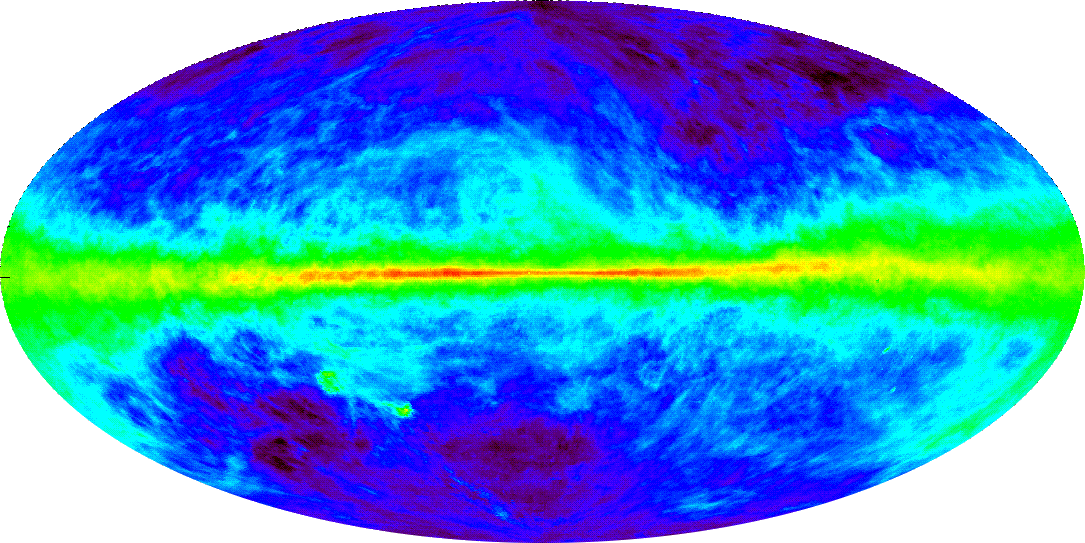
\includegraphics[width=\medpage]{images/21.png}
%%	\caption{Εκπομπή του \ce{HI} στα 21.1 cm (Kalberla et al., 2005)\cite{kalberla_2005}}
%%\end{figure}
%
%H καλύτερη μέχρι σήμερα δυνατή μέθοδος για την παρατήρηση του \textbf{Ουδέτερου Υδρογόνου \ce{H I}} είναι η εκπομπή της γραμμής $21.1 \, cm$ στα ραδιοκύματα που οφείλεται στη μετάπτωση αντιστροφής του spin του πρωτονίου και του ηλεκτρονίου στη βασική κατάσταση του ατόμου του Υδρογόνου. Η ενεργειακή διαφορά των καταστάσεων με συνολικό spin $F=1$ \textbf{(τα spin $p^+$ και $e^-$ είναι παράλληλα)} και $F=0$ \textbf{(τα spin $p^+$ και $e^-$ είναι άντιπαράλληλα)} είναι $h \nu=6\times 10^{-6} \, eV$, η οποία αντιστοιχεί στη γραμμή των 21 cm.
%Ο συντελεστής Einstein για την αυθόρμητη εκπομπή είναι $A_{10} \simeq 3\times 10^{-15}s^{-1}$ που αντιστοιχεί σε μια χρονική κλίμακα των $10^7$ ετών στην οποία παραμένει ένα διεγερμένο άτομο Υδρογόνου μέχρι να αποδιεγερθεί αυθόρμητα εκπέμποντας το παρατηρούμενο φωτόνιο. Ο πολύ μικρός αυτός ρυθμός εκπομπής αντιπαραβάλλεται εν τέλει από τη τεράστια ποσότητα του ατομικού υδρογόνου έτσι ώστε στατιστικά η γραμμή να είναι παρατηρήσιμη.
%
%\subparagraph{Εκπομπή \ce{H\alpha}}
%Κοντά σε αστέρες μεγάλης μάζας (φασματικού τύπου O και B) λόγω των φωτονίων υψηλής ενέργειας (μεγαλύτερες από το όριο Lyman) το αέριο υδρογόνο ιονίζεται. Οι περιοχές αυτές, ονομάζονται και Περιοχές HII, θα τις εξετάσουμε αναλυτικότερα στη παράγραφο~(\ref{par:HII regions}), και παρουσιάζουν έντονη εκπομπή ακτινοβολίας στη γραμμή Ha $(656.28\ nm)$ λόγω της επανασύνδεσης των ιονισμένων ατόμων.

%\begin{figure}[h]
%	\label{fig:Ha}
%	\centering
%	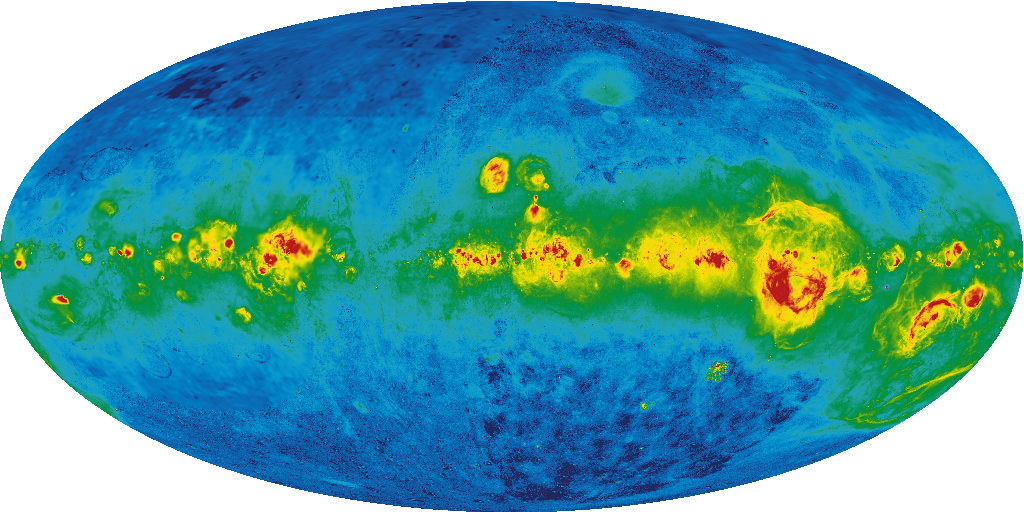
\includegraphics[width=\medpage]{images/Ha.png}
%	\caption{Εκπομπή Ha από συνδυασμό τριών διαφορετικών παρατηρήσεων (WHAM - VTSS - SHASSA) \cite{finkbeiner_2003}}
%\end{figure}
%

%===================================================================
%===================================================================
%===================================================================

\section{Μοριακά Νέφη}
%Οι πιο ενδιαφέρουσες, από τη σκοπιά της δημιουργίας αστέρων, περιοχές του Μεσοαστρικού Υλικού είναι τα Μοριακά Νέφη (Molecular Clouds).
Τα Μοριακά Νέφη είναι περιοχές όπου ψυχρή μεσοαστρική ύλη έχει πυκνότητες ικανοποιητικά μεγαλύτερες από τη μέση πυκνότητα του μεσοαστρικού υλικού έτσι η ιδιοβαρύτητα του νέφους να παίζει σημαντικό ρόλο στη δυναμική του. Καθώς το μοριακό νέφος καταρρέει, κατακρημνίζεται σε όλο και πιο συμπυκνωμένες δομές έως ότου η πυκνότητα και η μάζα σε μια τέτοια περιοχή είναι αρκετή ώστε να γεννηθούν νέοι αστέρες.   

\begin{marginfigure}
	\label{fig:CO}
	\centering
	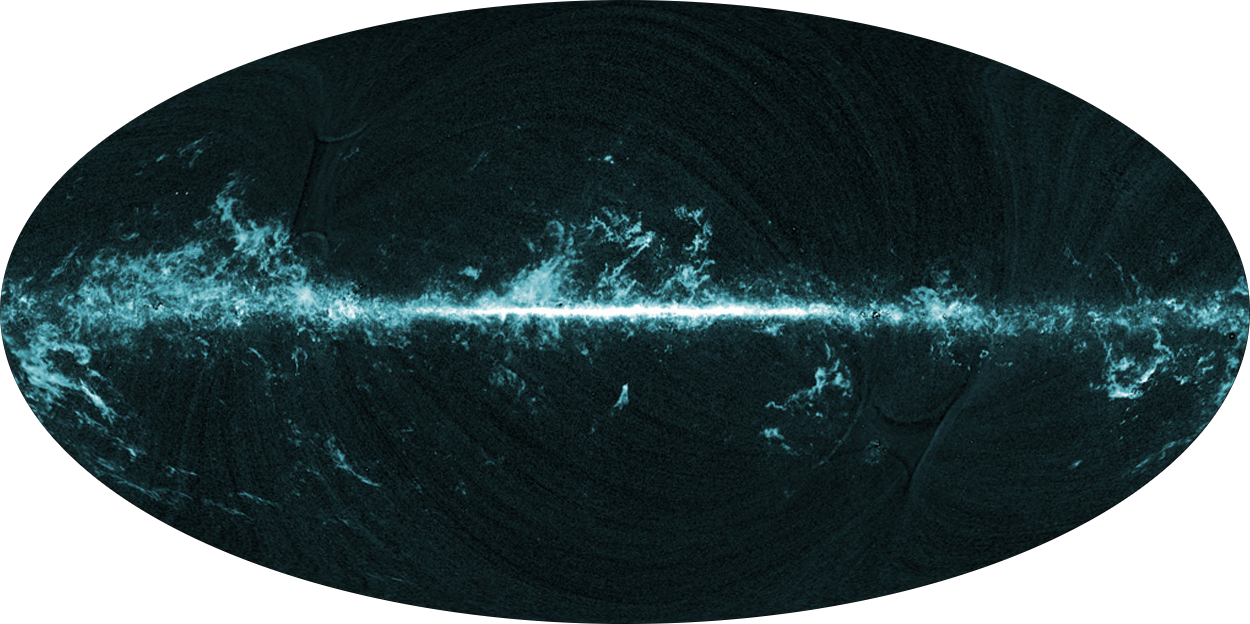
\includegraphics[width=1\linewidth]{Images/CO.png}
	\caption{Εκπομπή CO όπως τη χαρτογράφησε το Planck.\cite{planck_2014}.
		\newline
		Το \ce{H2} είναι ένα πλήρως συμμετρικό μόριο επομένως δεν έχει μόνιμη διπολική ροπή. Αυτό έχει σαν συνέπεια η διέγερση του να είναι σε θερμοκρασίες τις τάξεις των \SI{500}{K}. Άρα για τις τυπικές θερμοκρασίες των μοριακών νεφών $10-50\ K$ είναι αδύνατον να το παρατηρήσουμε άμεσα.
		\newline
		Ο εναλλακτικός τρόπος παρατήρησης του \ce{H2} είναι εμμέσως μέσω της εκπομπής διαφορετικών μορίων που είναι πιο "ευαίσθητα" στις χαμηλές θερμοκρασίες, όπως του \ce{CO} που είναι το δεύτερο σε αναλογία μόριο στο Σύμπαν και έχει μόνιμη διπολική ροπή (άρα έχουμε περιστροφικές ενεργειακές μεταβάσεις) πράγμα του επιτρέπει να εκπέμπει σημαντικά στο ραδιοφωνικό φάσμα.. 
		\newline
		H χαμηλότερη μετάβαση αντιστοιχεί σε θερμοκρασία \SI{5.5}{K} και αποδίδει ένα ραδιοφωνικό φωτόνιο στα \SI{2.6}{mm}.
	}
	%
	%Ο κύριος μηχανισμός διέγερσης ενός μορίου \ce{CO} στη $J=1$ είναι μέσω της σύγκρουσης του με ένα μόριο \ce{H2}. Αφού διεγερθεί η αποδιέγερση του μπορεί να γίνει είτε εκπέμποντας ένα φωτόνιο στα \SI{2.6}{mm} σε περιοχές με χαμηλή συνολική πυκνότητα είτε μεταφέροντας την ενέργεια του σε ξανά σε ένα μόριο \ce{H2} χωρίς να εκπεμφθεί φωτόνιο σε περιοχές με μεγάλη συνολική πυκνότητα.
	
\end{marginfigure}

Όπως φαίνεται και από το όνομα τους, τα Μοριακά Νέφη αποτελούνται κυρίως από μοριακό Υδρογόνο \ce{H2}. Στο γαλαξία μας πάνω από το 80\% του μοριακού Υδρογόνου βρίσκεται σε μοριακά νέφη κατανεμημένα πάνω στις σπείρες του δίσκου αλλά κυρίως σε ένα δακτύλιο ακτίνας 3 με 5 kpc από το κέντρο του γαλαξία \cite{rathborne_2009}.  Από παρατηρήσεις στο \ce{CO} τα μοριακά νέφη δείχνουν να έχουν μάζες που κυμαίνονται από \SIrange{1e3}{1e6}{M_\odot} με μια κατανομή νόμου δύναμης $-1.6$. \cite{stahlern_2004}

Για να δημιουργηθεί το Μοριακό Υδρογόνο καταλυτικό ρόλο παίζει η μεσοαστρική σκόνη.  Όταν δύο άτομα Υδρογόνου ενώνονται και δημιουργούν ένα μόριο \ce{H2} αυτό κερδίζει ενέργεια η οποία όμως δεν μπορεί να αποδοθεί στο περιβάλλον με αποτέλεσμα το μόριο να διασπάται. Παρολαυτά αν η διαδικασία αυτή γίνει πάνω σε έναν κόκκο σκόνης, τότε αυτός λειτουργεί καταλυτικά απορροφώντας το πλεόνασμα ενέργειας και το μόριο παραμένει σταθερό. Έτσι το ουδέτερο Υδρογόνο λειτουργεί σαν καύσιμο που τροφοδοτεί τις πυκνότερες περιοχές του μοριακού Υδρογόνου.

Ένα τυπικό μοριακό νέφος επιβιώνει για \SI{3e7}{yrs} πριν καταστραφεί από τους βίαιους αστρικούς ανέμους των αστέρων τύπου O και B που έχουν δημιουργηθεί στο εσωτερικό του. Κατά τη διάρκεια της ζωής του το νέφος αποδίδει τελικά ένα 3\% της μάζας του σε αστέρες. Έτσι για παράδειγμα αν θεωρήσουμε μια τιμή της συνολικής μάζας του μοριακού \ce{H2} στο Γαλαξιακό δίσκο \SI{2e9}{M_\odot} βρίσκουμε ότι ο ρυθμός δημιουργίας αστέρων (SFR) για το Γαλαξία μας είναι περίπου \SI{2}{M_\odot} ανά έτος.  


\begin{table}
	\caption{Χαρακτηριστικά και διαφορετικοί τύποι Μοριακών Νεφών}
	\label{tab:MCtypes}
	\begin{tabular}{l c c c c}
		\toprule
		\multirow{2}{*}{Κατηγορία} & Μέση ακτίνα &  Θερμοκρασία & Πυκνότητα \ce{H2} & Μάζα \\ 
		& \si{(pc)} & \si{(K)} & \si{(cm^{-3})} & \si{(M_\odot)} \\
		\midrule
		Γιγαντιαίο Μοριακό Νέφος & \num{20} & \num{15} & \num{100} & \num{1e5} \\
		Μοριακό Νέφος & $5$ & $10$ & $300$ & $10^4$\\
		clump & $2$ & $10$ & $10^3$ & $10^3$\\
		Πυρήνας Νέφους & $0.08$ & $10$ & $10^5$ & $10$\\
		\bottomrule
	\end{tabular}
\end{table}


%\subsection{Ενεργειακή ισορροπία στα Μοριακά Νέφη}
%Όπως αναφέραμε γενικότερα στη παράγραφο~(\ref{par:EnergyBalance}) η θερμοκρασία ενός νέφους είναι αποτέλεσμα στης ενεργειακής ισορροπίας μεταξύ των μηχανισμών θέρμανσης και ψύξης. Για τα Μοριακά Νέφη συγκεκριμένα η θέρμανση είναι αποτέλεσμα της θερμότητας που παρέχεται από κοντινά άστρα ή μέσω της κοσμικής ακτινοβολίας, ενώ η ψύξη επιτυγχάνεται μέσω διαδικασιών απορρόφησης και κρούσης με τα σωματίδια της σκόνης ή του αερίου.
%Η ενέργεια τελικά αποδίδεται μέσω της υπέρυθρης ακτινοβολίας η οποία οφείλεται στην απορρόφηση και την εκπομπή των φωτονίων από το περιβάλλοντα αέριο και σκόνη.
%

\section{Ενεργειακή ισορροπία}
\label{par:EnergyBalance}
Η κινητική θερμοκρασία \footnote{Το ψυχρό μεσοαστρικό αέριο λόγω της γενικά χαμηλής του πυκνότητας δεν βρίσκεται σε θερμοδυναμική ισορροπία. Επομένως όταν μιλάμε για θερμοκρασία αναφερόμαστε στη κινητική του θερμοκρασία.\cite[p. 28]{spitzer_1998}} της Μεσοαστρικής Ύλης κυμαίνεται σε ένα εύρος τιμών 6 τάξεων μεγέθους όπως παρατηρούμε και από τον πίνακα~\ref{tab:ISM}. Για να περιγράψουμε και να μοντελοποιήσουμε την ενεργειακή ισορροπία στη Μεσοαστρική Ύλη και άρα να εξηγήσουμε και τις παρατηρούμενες θερμοκρασίες θα πρέπει να υπολογίσουμε τις διαδικασίες θέρμανσης και ψύξης. 
%Ενώ η κύρια διαδικασία ψύξης είναι η εκπομπή ακτινοβολίας είτε μέσω αυθόρμητης αποδιέγερσης ή αποδιέγερσης λόγω κρούσης, για τη θέρμανση έχουμε μια πληθώρα διαδικασιών οι οποίες μπορούν να ταξινομηθούν σε 3 κατηγορίες:
%
%\begin{itemize}
%	\item θέρμανση από πεδία ακτινοβολίας: φωτοηλεκτρική απορρόφηση σε ουδέτερα στοιχεία, φωτοδιάσπαση στα μόρια, φωτοιονισμός.
%	\item θέρμανση μέσω συγκρούσεων: από τυρβώδες ροές, κρουστικά κύματα καταλοίπων supernova και κοσμικής ακτινοβολίας.
%	\item θερμική ανταλλαγή μεταξύ της σκόνης και νεφών αερίου, αλληλεπίδραση ιονισμένου αερίου με μαγνητικά πεδία, βαρυτική κατάρρευση. 
%\end{itemize}

%=======ΦΩΤΗΣ==================
Ο πιο γενικός διαχωρισμός των μηχανισμών θέρμανσης και ψύξης αφορά τις διαδικασίες που έχουν να κάνουν με θέρμανση λόγω φώτο-ιονισμού και διαδικασίες ψύξης λόγω διέγερσης από αλληλεπίδραση μεταξύ σωματιδίων. Παρακάτω θα παρουσιαστεί μια διαισθητική εικόνα των διαδικασιών αυτών.
\begin{itemize}
	\item \textbf{Φώτο-ιονισμός ουδέτερων ατόμων} \\
	Ένα φωτόνιο προσπίπτει σε ένα ουδέτερο άτομο επάγοντας τον ιονισμό του. Έχουμε λοιπόν ένα ελεύθερο ηλεκτρόνιο με ενέργεια $E$ το οποίο μέσω συγκρούσεων με άλλα ουδέτερα σωμάτια του αερίου μεταφέρει ενέργεια στο αέριο, θερμαίνοντας το. Ωστόσο, λόγω επανασύνδεσης (recombination) η αποδιδόμενη ενέργεια είναι μικρότερη απο την αρχική ενέργεια του ηλεκτρονίου.
	\item \textbf{Αλληλεπιδράσεις μεταξύ σωματιδίων} \\ Ελεύθερα σωματίδια αλληλεπιδρούν μέσω κρούσεων επάγοντας μεταβάσεις σε διεγερμένες ενεργειακές στάθμες. Κατά τις συνεπακόλουθες μεταβάσεις στην βασική κατάσταση εκπέμπονται φωτόνια, τα οποία εφόσον διαφύγουν από την περιοχή αντιστοιχούν σε απώλεια ενέργειας.
	Ακολουθεί μια αυστηρότερη περιγραφή των παραπάνω διεργασιών.
	% θελει πιο ομορφη περιγραφη, μοιαζει με κείμενο πενταχρονου
\end{itemize}
\subsection{Θερμοδυναμική περιγραφή}
Ξεκινάμε από τον πρώτο νόμο τις θερμοδυναμικής:
\begin{equation}
dE = \bar{d}Q - dW
\end{equation}
Όπου $dE$ η μεταβολή της εσωτερικής ενέργειας, $\bar{d}Q$ η θερμότητα που απορρόφησε το σύστημα και $dW$ το έργο που έγινε από το σύστημα.

% Για ημιστατικό σύστημα έχουμε οτι $\bar{d}Q = TdS$, $dS$ το διαφορικό της εντροπίας και επίσης απο τον ορισμό του έργου, $dW=pdV$ όπου $dV$ η μεταβολή του όγκου του συστήματος και $p$ η πίεση.
%
%\begin{equation}
%TdS =dE +pdV
%\end{equation}
Για ιδανικά αέρια, η εσωτερική ενέργεια εξαρτάται μόνο απο τη θερμοκρασία και η καταστατική εξίσωση γράφεται ως: $p=nk_bT$, όπου $k_b$ η σταθερά του Boltzmann και $n$ η αριθμητική πυκνότητα του αερίου. Ακολούθως, 
χρησιμοποιώντας το ότι η εσωτερική ενέργεια μονατομικού ιδανικού αερίου είναι $E = \frac{3}{2}NkT$ η απορροφούμενη θερμότητα ανά μονάδα όγκου είναι:

\begin{equation}
\frac{dQ}{V}=nd\left(\frac{3}{2}kT \right)-kTdn
\end{equation}

Στη γενικότητα, οι διαδικασίες θέρμανσης και ψύξης εξαρτώνται από τον χρόνο και η ολική ενέργεια ανά μονάδα όγκου ανά μονάδα χρόνου ισούται με:
\marginpar{
	Στην σχέση \ref{eq:CoolingHeating} αγνοήσαμε τη θερμική αγωγιμότητα η οποία δεν παίζει ιδιαίτερο ρόλο στις τυπικές θερμοκρασίες του μεοαστρικού υλικού $T< 2\cdot 10^{4}K$. Γενικά θα έπρεπε να προσθέσουμε στο αριστερό μέλος την ποσότητα $\nabla \cdot (K\nabla T) $ όπου $K$ η θερμική αγωγιμότητα. Εδώ θα πρέπει να σημειωθεί ότι σε περιοχές υψηλών θερμοκρασιών, η παρουσία μαγνητικών πεδίων επηρεάζει επιπλέον την θερμική αγωγιμότητα.
}

\begin{equation}
\label{eq:CoolingHeating}
\Delta = n\frac{d}{dt}\left(\frac{3}{2}kT \right)-kT\frac{dn}{dt}
\end{equation}


Έστω τώρα ότι η θερμότητα ανά μονάδα όγκου και χρόνου που προστίθεται στο αέριο από την αλληλεπίδραση των σωματιδίων $\xi,n$ είναι $\Gamma_{\xi \eta}$ και όμοια, η συνεισφορά των αλληλεπιδράσεων αυτών στην ψύξη είναι $\Lambda_{\xi \eta} $. Ορίζουμε τις συναρτήσεις ψύξης (cooling function) και θέρμανσης (heating function) ως:

\begin{equation}
\Lambda = \sum_{\xi \eta}\Lambda_{\xi \eta}
\label{thermFunction}
\end{equation}

\begin{equation}
\Gamma = \sum_{\xi \eta}\Gamma_{\xi \eta}
\end{equation}
Συνεπώς έχουμε ότι:
\begin{equation}
\Delta = \Gamma -\Lambda
\end{equation}
Μπορούμε να δούμε ότι αν η αριθμητική πυκνότητα και η θερμοκρασία δεν μεταβάλλονται με τον χρόνο ισχύει ότι 
\begin{equation}
\Delta = 0 \Rightarrow \Gamma = \Lambda 
\end{equation}
Με βάση τη τελευταία σχέση μπορούμε να ορίσουμε τη \emph{θερμοκρασία ισορροπίας}. Για τον ορισμό της τελευταίας χρειάζεται να γνωρίζουμε όλους τους μηχανισμούς θέρμανσης και ψύξης του αερίου. Στο υπόλοιπο κείμενο θα θεωρήσουμε οτι το αέριο βρίσκεται στη θερμοκρασία σταθερής κατάστασης εκτός και αν αναφέρεται κάτι διαφορετικό. Εν συνεχεία θα παρουσιάσουμε τις συναρτησεις ψύξης/θέρμανσης για διάφορες φυσικές διαδικασίες.

% % % % % % % 
%Εδώ πρέπει να συζητηθεί η %χρονική κλίμακα των %transient φαινομένων.
\subsection{Μηχανισμοί Θέρμανσης}
\subsubsection{Κοσμική ακτινοβολία}
Ένας πολύ σημαντικός μηχανισμός θέρμανσης της μεοαστρικής ύλης και κατα συνέπεια και των μοριακών νεφών είναι η κοσμική ακτινοβολία. Η κοσμική ακτινοβολία αποτελείτε επί το πλείστον από σχετικιστικά πρωτόνια μαζί με λιγότερα βαρύτερα στοιχεία ή ηλεκτρόνια. Η ενεργειακή κατανομή των κοσμικών αυτών σωματιδίων κυμαίνεται από ενέργειες των \SIrange{10}{1e14}{MeV} με κατανομή νόμου δύναμης $\Phi _\mathtt{CR}(E)\sim E^{-2.7}$ (για τη ροή) (βλέπε και σχήμα \ref{fig:crenergy}).

%\paragraph{Αλληλεπίδραση Κοσμικής ακτινοβολίας με μοριακό αέριο}
Κατά την αλληλεπίδραση ενός πρωτονίου της κοσμικής ακτινοβολίας με το μοριακό υδρογόνο ενός μοριακού νέφους είτε το \ce{H2} θα διεγερθεί και θα διασπαστεί σε δύο Υδρογόνα είτε θα έχουμε απευθείας ιονισμό. Ξεκινώντας από τον ιονισμό έχουμε την αντίδραση:
\begin{marginfigure}
	\centering
	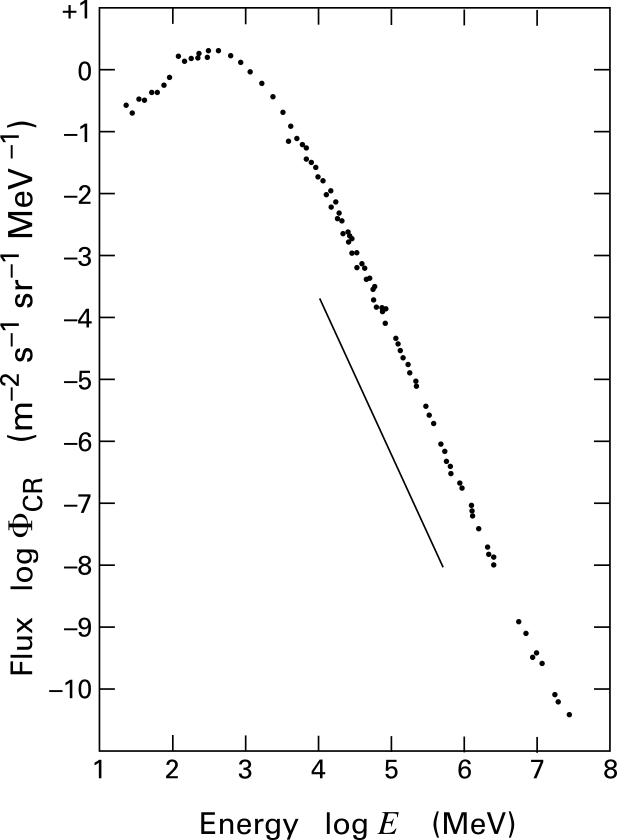
\includegraphics[width=1\linewidth]{Images/CRenergy}
	\caption{}
	\label{fig:crenergy}
\end{marginfigure}

\begin{equation}
\ce{p^+ +H2 -> H2 ^+ +e^- +p^+}
\end{equation}
Καθώς το ηλεκτρόνιο που διαφεύγει αλληλεπιδρά με τα γειτονικά μοριακά υδρογόνα θερμαίνει το αέριο με ρυθμό
\begin{equation}
\Gamma _\mathtt{CR} (\ce{H2}) =\zeta (\ce{H2})n_{\ce{H2}} \Delta E (\ce{H2})
\end{equation}
όπου $\zeta (\ce{H2})$ είναι ο ρυθμός ιονισμού ενός μορίου \ce{H2}, $n_{\ce{H2}}$ η αριθμητική πυκνότητα του μοριακού υδρογόνου και $\Delta E (\ce{H2})$ η θερμική ενέργεια που προσδίδεται στο αέριο σε κάθε ιονισμό. Η ενέργεια αυτή εξαρτάται από την ενέργεια του κοσμικού πρωτονίου. Πρωτόνια με ενέργεια μεγαλύτερη του \SI{1}{GeV} διεγείρουν το πυρήνα με αποτέλεσμα την εκπομπή ακτίνων γ και δεν εναποθέτουν ενέργεια στο αέριο. Παίρνοντας μια τυπική για το πρωτόνιο τιμή των \SI{10}{MeV} η ενέργεια που αποδίδεται στο ηλεκτρόνιο είναι \SI{30}{eV}. 

Το ηλεκτρόνιο τώρα μπορεί είτε να ιονίσει περαιτέρω το μοριακό αέριο μέσω της
\begin{equation}
\ce{e^- + H2 -> H2^+ + e^- + e^-}
\end{equation}
η οποία δεν προσδίδει θέρμανση αλλά εμπλουτίζει το χώρο με περισσότερο ενεργητικά ηλεκτρόνια ή να θερμάνει τελικά το αέριο μέσω της διάσπασης του μορίου
\begin{equation}
\ce{e^- + H2 -> H + H + e^-}
\end{equation} 
Κάνοντας το λεπτομερή υπολογισμό μέσω του δικτύου όλων τα πιθανών σεναρίων βρίσκουμε ότι η ενεργειακή ενέργεια ανά ιονισμό είναι $\Delta E (\ce{H2}) = \SI{7}{eV}$. Η τιμή αυτή δεν εξαρτάται σημαντικά από την ενέργεια του κοσμικού πρωτονίου, ενδεικτικά η τιμή του $\Delta E (\ce{H2})$ για ενέργειες πρωτονίων \SIrange{1}{100}{MeV} κυμαίνεται αντίστοιχα στα \SIrange{6.3}{7.6}{eV}.

Στη περίπτωση της αλληλεπίδρασης της κοσμικής ακτινοβολίας με ουδέτερο Υδρογόνο ο ιονισμός πραγματοποιείται μέσω της:
\begin{equation}
\ce{p^+ + H -> H^+ + e^- + p^+}
\end{equation}
όπου το ηλεκτρόνιο τώρα δραπετεύει με ενέργεια στα \SI{35}{eV} συνεισφέροντας με ρυθμό θέρμανσης αντίστοιχα με πριν
\begin{equation}
\Gamma _\mathtt{CR} (\ce{HI}) =\zeta (\ce{HI})n_{\ce{HI}} \Delta E (\ce{HI})
\end{equation}

Η ενέργεια του ηλεκτρονίου είναι όμως αρκετά υψηλή ώστε για να θερμάνει το αέριο, με αποτέλεσμα τα διεγερμένα ή ιονισμένα άτομα να ατκινοβολούν το πλεόνασμα. Τελικά η θέρμανση θα ξεκινήσει όταν το ηλεκτρόνιο αποχτήσει ενέργεια κάτω από \SI{10.2}{eV} η οποία αντιστοιχεί στη πρώτη διεγερμένη στάθμη του υδρογόνου ($n=2$). Έπειτα από αριθμητικούς υπολογισμούς η ενέργεια ανά ιονισμό $\Delta E (\ce{HI})$ υπολογίζεται στα \SI{6}{eV}.

Ο υπολογισμός των ρυθμών ιονισμού $\zeta (\ce{H2}),\zeta (\ce{HI})$ μπορεί να εκτιμηθεί μέσω παρατηρήσεων. Καθώς το ιονισμένο από τις κοσμικές ακτίνες υδρογόνο αντιδρά με γειτονικά μόρια ξεκινά μια αλληλουχία αντιδράσεων που έχουν σαν αποτέλεσμα όλο και πιο πολύπλοκες ενώσεις. Έτσι παρατηρώντας τις αναλογίες αυτών των ενώσεων μπορούμε να κάνουμε μια εκτίμηση για το ρυθμό ιονισμού.

Αν πάρουμε για παράδειγμα την αλληλεπίδραση του ιονισμένου υδρογόνου με το οξυγόνο έχουμε την ακόλουθη αλληλουχία αντιδράσεων
\begin{align}
\ce{H^+ + O &-> O^+ + H} \\
\ce{O^+ + H2 &-> OH^+ + H}\\
\ce{OH ^+ + H2 &-> H2O^+ + H}\\
\ce{H2O^+ + H2 &-> H3O^+ + H}
\end{align}

Το \ce{H3O^+} δεν μπορεί να δεχτεί παραπάνω υδρογόνα άρα κατά την επανασύνδεση έχει δύο πιθανά αποτελέσματα
\begin{align}
\ce{H3O^+ + e^- &-> OH + H2} \\
\ce{H3O^+ + e^- &-> H2O + H}
\end{align}
με τη πρώτη αντίδραση να είναι πιο πιθανή με πιθανότητα από εργαστηριακές μετρήσεις να είναι $p=\num{0.75}$. Στη στατική κατάσταση όπου ο ρυθμός  δημιουργίας \ce{OH} $p  \zeta (\ce{HI}) n_{\ce{HI}}$ είναι ίδιος με το ρυθμό καταστροφής του $\frac{n_{\ce{OH}}}{\tau _\mathtt{photo}}$ με $\tau _\mathtt{photo}$ να είναι ο χαρακτηριστικός χρόνος φωτοδιάσπασης από τα υπεριώδη φωτόνια με τυπική τιμή στα διάχυτα νέφη \SI{2e10}{s}.

Άρα αντικαθιστώντας τη παρατηρησιακή τιμή της σχετικής αναλογίας του \ce{OH} (μέσω γραμμών απορρόφησης στο υπεριώδες) $\frac{n_{\ce{OH}}}{n_{\ce{H}}} = \num{2e-7}$ βρίσκουμε
\begin{equation}
\zeta (\ce{HI}) = \frac{n_{\ce{OH}}}{n_{\ce{H}}} \left(p \tau _\mathtt{photo} \right) ^{-1} = \SI{2e-17}{s^{-1}}
\end{equation}

Για τον ιονισμό του μοριακού υδρογόνου θεωρητικοί υπολογισμοί δίνουν ότι η πιθανότητα ιονισμού είναι \num{1.6} φορές σε σχέση με το ατομικό υδρογόνο. Περνώντας υπόψιν και τις διορθώσεις από τους δευτερεύων ιονισμούς έχουμε τελικά:
\begin{equation}
\zeta (\ce{H2})=\SI{3e-17}{s^{-1}}
\end{equation}

Άρα τελικά οι ρυθμοί θέρμανσης θα είναι
\begin{align}
\Gamma _\mathtt{CR} (\ce{HI}) &= \num{1.6e-25} \left( \frac{n_{\ce{HI}}}{\SI{1e3}{cm^{-3}}} \right) \qq{(\si{erg.cm^{-3}.s^{-1}})} \\
\Gamma _\mathtt{CR} (\ce{H2}) &= \num{3.2e-25} \left( \frac{n_{\ce{H2}}}{\SI{1e3}{cm^{-3}}} \right) \qq{(\si{erg.cm^{-3}.s^{-1}})} 
\end{align}

\subsubsection{Διάχυτη ακτινοβολία}

Ένας δεύτερος μηχανισμός θέρμανσης του μεσοαστρικού αερίου είναι η διάχυτη ακτινοβολία. Όπως βλέπουμε κι από το σχήμα \ref{fig:interstellarradiation} με τη μέση ένταση της αστρικής ακτινοβολίας για τη γειτονιά του Ήλιου. 

Τα πρώτο από τα τρία μέγιστα που παρατηρούμε αντιστοιχεί στο κοσμικό υπόβαθρο (\SI{11.3}{Hz}) με μια κατανομή μέλανος σώματος που αντιστοιχεί στους \SI{2.74}{K} απόηχο της μεγάλης έκρηξης. Τα φωτόνια του κοσμικού υποβάθρου θερμαίνουν τα μοριακά νέφη διεγείροντας τις χαμηλότερες περιστροφικές ενεργειακές στάθμες του \ce{CO}.

\begin{marginfigure}
	\centering
	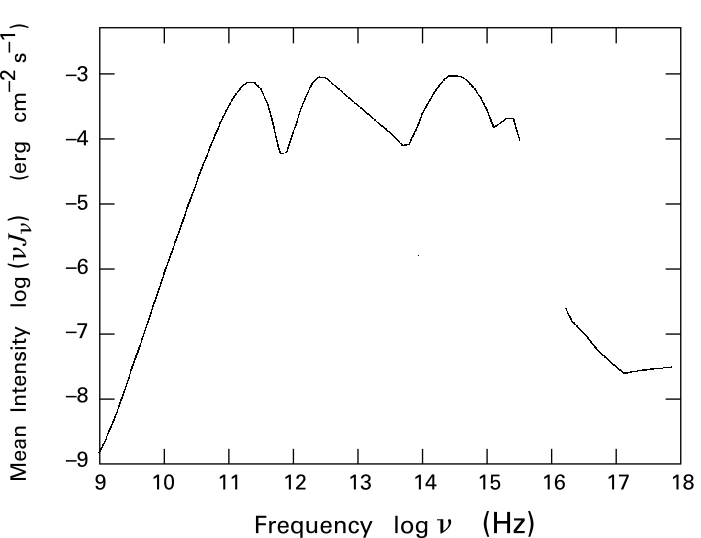
\includegraphics[width=1\linewidth]{Images/interstellarradiation}
	\caption{}
	\label{fig:interstellarradiation}
\end{marginfigure}

Το επόμενο μέγιστο (\SI{12.4}{Hz}) προέρχεται από την εκπομπή των κόκκων σκόνης στο βαθύ υπέρυθρο καθώς αυτοί θερμαίνονται από την αστρική ακτινοβολία. Αν και με το μηχανισμό αυτό θα ασχοληθούμε ξανά στη συνέχεια, \todo{σιγουρα?} η συγκεκριμένη ακτινοβολία δεν προσφέρει θέρμανση στα μοριακά νέφη καθώς δεν αλληλεπιδρά μαζί τους.

Το τελευταίο μέγιστο (\SI{14.5}{Hz}) στο οπτικό μέρος του φάσματος αντιστοιχεί στην ακτινοβολία από τους αστέρες. Αν προσεγγίσουμε την ακτινοβολία αυτή με μια κατανομή μέλος σώματος βρίσκουμε μια ενεργό θερμοκρασία $\bar{T}=\SI{5400}{K}$ η οποία αντιστοιχεί σε ένα αστέρα φασματικού τύπου G3 με παράμετρο μείωσης $A=\Omega/4\pi= \num{1e-13}$, όπου $\Omega$ η στερεά γωνία που θα καταλαμβάνε ο "αστερας" αυτός στον ουρανό.

Στη συνέχεια έχουμε ένα μικρότερο μέγιστο (\SI{15.3}{Hz}) στο υπεριώδες που αντιστοιχεί στους πολύ θερμούς αστέρεςς και μπορεί αντίστοιχα να προσεγγιστεί από ένα μέλαν σώμα θερμοκρασίας $\bar{T}=\SI{3.4e4}{K}$ και παράμετρο μείωσης  $\Omega/4\pi= \num{1e-17}$. 

Η ακτινοβολία στις μεγαλύτερες συχνότητες σχετίζεται με εκπομπή του υπέρθερμου αερίου με θερμοκρασίες της τάξης των \SI{1e6}{K} που όπως είπαμε και προηγουμένως θερμαίνεται από κρουστικά κύματα εκρήξεων supernovae και βίαιους αστρικών ανέμους. 

Παρακάτω θα επικεντρωθούμε στη θέρμανση από τη κοσμική ακτινοβολία και το διάχυτο πεδίο ακτινοβολίας και θα αποφύγουμε να μιλήσουμε για την επίδραση των ίδιων των αστέρων που δημιουργούνται εντός των μοριακών νεφών. Ενδεικτικά, αν θεωρήσουμε ότι οι αστέρες αυτοί δεν συμπεριλαμβάνονται στο πεδίο ακτινοβολίας που αναφέρουμε παραπάνω επιδρούν μέσω της ακτινοβολίας στο υπεριώδες και τις ακτίνες Χ (δημιουργία των περιοχών \ce{HII}).

\paragraph{Ιονισμός Άνθρακα}
Η ένταση στο υπεριώδες τμήμα της ακτινοβολίας είναι αρκετά χαμηλή στις ενέργειες πάνω από \SI{13.6}{eV} ώστε ο ιονισμός του Υδρογόνου να είναι σημαντικός.\todo{εξαιρεση περιοχες HII} Όμως μια σειρά από βαρύτερα στοιχεία έχουμε χαμηλότερες ενέργειες ιονισμού. Το πιο συχνό από αυτά είναι ο ατομικός άνθρακας (\ce{CI}) με αριθμητική αναλογία $\frac{n_{\ce{CI}}}{n_{\ce{H}}} =\num{3e-4}$ και ενέργεια ιονισμού στα \SI{11.2}{eV}.  Ο μηχανισμός θέρμανσης είναι ανάλογος με προηγουμένως δίνοντας ένα ρυθμό θέρμανσης:
\begin{equation}
\Gamma _\mathtt{IR} (\ce{CI}) =\zeta (\ce{CI})n_{\ce{C}} \Delta E (\ce{CI})
\end{equation}
 με $\zeta (\ce{CI})$ το ρυθμό ιονισμού και $\Delta E (\ce{CI})$ τη μέση ενέργεια του εξεγερμένου \todo{!!!} ηλεκτρονίου.
 
 Ολοκληρώνοντας τη μέση ένταση ακτινοβολίας $J_{\nu}$ στις συχνότητες που μας ενδιαφέρουν και πολλαπλασιάζοντας με την ενεργό διατομή ιονισμού του \ce{CI} βρίσκουμε 
 \begin{align}
\zeta (\ce{CI}) =\SI{1e-10}{s^{-1}} && \Delta E (\ce{CI})=\SI{1}{eV}
 \end{align}
 άρα βρίσκουμε τελικά για το ρυθμό θέρμανσης, χρησιμοποιώντας και τη σχετική αναλογία του \ce{CI} 
 
 \marginpar{Αξίζει να σημειωθεί ότι η τιμή για το $\Gamma _\mathtt{IR} (\ce{CI})$ είναι μέγιστη καθώς προϋποθέτει ότι όλη η ποσότητα του άνθρακα είναι σε ουδέτερη μορφή. Στη πράξη στις περιοχές όπου η θέρμανση είναι σημαντική, το ποσοστό ιονισμού του άνθρακα είναι μεγάλο άρα η τιμή για τη $\Gamma _\mathtt{IR} (\ce{CI})$ θα είναι σαφως μικρότερη}
 
  \begin{equation}
 \Gamma _\mathtt{IR} (\ce{CI}) = \num{6.41e-23} \left( \frac{n_{\ce{H}}}{\SI{1e3}{cm^{-3}}} \right) \qq{(\si{erg.cm^{-3}.s^{-1}})} 
 \end{equation}
 
\paragraph{Διέγερση Μοριακού Υδρογόνου}
Ένα φωτόνιο ενέργειας \SI{11.2}{eV} διεγείρει ένα μόριο \ce{H2}. Το διεγερμένο μόριο είτε θα επανέρθει στη βασική κατάσταση μέσω της εκπομπής ακτινοβολίας στο υπέρυθρο και υπεριώδες είτε θα διασπαστεί εκπέμποντας ένα φωτόνιο ενέργειας $h \nu - \Delta E _\mathtt{diss} -\epsilon$ όπου $\epsilon$ η κινητική ενέργεια που θα διαχυθεί στα γειτονικά άτομα. Η τιμή της $\epsilon$ κυμαίνεται στα περίπου \SI{2}{eV}. 

Επειδή όμως το μοριακό υδρογόνο δεν είναι εκτεθειμένο στο διαστρικό πεδίο ακτινοβολίας ο μηχανισμός αυτός δεν αποδίδει τελικά στη θέρμανση του νέφους.

\paragraph{Θέρμανση Κόκκων σκόνης}
Τα υπεριώδη φωτόνια επίσης μπορούν να διεγείρουν ηλεκτρόνια και από τους κόκκους σκόνης τα οποία στη συνέχεια θερμαίνουν το γειτονικό αέριο. Ένα φωτόνιο μπορεί να εισχωρήσει μέχρι μια απόσταση \SI{100}{\angstrom} εντός του κόκκου έως ότου αποδεσμεύσει ένα ηλεκτρόνιο. Από τα ηλεκτρόνια που θα αποδεσμευτούν μόνο ένα 10\% θα φτάσει στην επιφάνεια και ένα ποσοστό απο αυτά θα έχει την απαιτούμενη ενέργεια που χρειάζεται για να αποδεσμευτεί από την επιφάνεια του κόκκου που είναι περίπου \SI{6}{eV}. Τελικά η ενέργεια του ελεύθερου ηλεκτρονίου είναι τη τάξης του \SI{1}{eV} άρα μπορούμε να πούμε ότι ο συντελεστής ενεργειακής απόδοσης $\epsilon _\mathtt{PE}$ είναι περίπου \num{0.01}. Παρόλο τη μικρή ενεργειακή απόδοση η θέρμανση είναι σημαντική λόγο του μεγάλου μεγέθους των κόκκων. Έτσι μπορούμε να υπολογίσουμε το ρυθμό θέρμανσης:
\begin{equation}
\Gamma _\mathtt{PE}=4\pi n_\mathtt{d} \sigma _\mathtt{d} \epsilon _\mathtt{PE} \int _\mathtt{FUV} J_\nu d\nu
\end{equation}  
όπου ολοκληρώνουμε στις ενέργειες πάνω από \SI{6}{eV} και ο παράγοντας $4\pi$ προέρχεται από τη παραδοχή ότι η ειδικής ένταση της ακτινοβολίας είναι ισοτροπική και οι κόκκοι έχουν σφαιρικό σχήμα. 

Με βάση θεωρητικές και εμπειρικές εκτιμήσεις μπορούμε να υπολογίσουμε τη ποσότητα $\Sigma _\mathtt{d} = n_\mathtt{d} \sigma _\mathtt{d}/n_{\ce{H}}$ στα \SI{1.5e-21}{cm^2} ενώ από παρατηρήσεις βρίσκουμε τη λεγόμενη "ροή Habing" $4\pi \int _\mathtt{FUV} J_\nu d\nu$ στα \SI{1.6e-3}{erg.cm^{-2}s^{-1}}. Άρα τελικά:
	
\begin{equation}
\Gamma _\mathtt{PE} = \num{4.8e-23} \left( \frac{n_{\ce{H}}}{\SI{1e3}{cm^{-3}}} \right) \qq{(\si{erg.cm^{-3}.s^{-1}})} 
\end{equation}

Το ποσοστό των ηλεκτρονίων που δεν καταφέρνουν να διαφύγουν ανεβάζουν τη θερμοκρασία του ίδιου του κόκκου $T_\mathtt{d}$. Στο μηχανισμό αυτό συμμετέχουν και τα οπτικά φωτόνια, που λόγο της πολύ μεγαλύτερης ροής μπορούμε να θεωρήσουμε αμελητέα πια τη ροή στο υπεριώδες. Έτσι έχουμε για τη θέρμανση των κόκκων:
\begin{equation}
\Gamma _\mathtt{d}=4\pi n_\mathtt{d} \sigma _\mathtt{d} \int _\mathtt{VIS} Q_\mathtt{abs}(\nu) J_\nu d\nu
\end{equation}  
 με $Q_{\nu,\mathtt{abs}}$ να είναι ο συντελεστής απορρόφησης ο οποίος στο οπτικό είναι ανάλογος του $\nu$. Αν θεωρήσουμε το πεδίο ακτινοβολίας $J_\nu$ σαν μέλαν σώμα θερμοκρασίας $\bar{T}$ με μέγιστο στη συχνότητα $\nu _\mathtt{max}$ θα έχουμε
  \begin{equation}
 \Gamma _\mathtt{d}=4\pi n_\mathtt{d} \sigma _\mathtt{d} A Q_{\nu _\mathtt{max}} 
					 \int _0 ^\infty \left( \frac{\nu}{\nu _\mathtt{max}}\right) 
					 \frac{2h\nu ^3/c^2}{e^{h\nu/k_B \bar{T}}} d\nu
 \end{equation}
 
 Αντικαθιστώντας όπως προηγουμένως και χρησιμοποιώντας για τη $Q_{\nu _\mathtt{max}}$ τη τιμή \num{0.1} για $\nu _\mathtt{max} =\SI{3e14}{s^{-1}}$ βρίσκουμε:
 \begin{equation}
 \Gamma _\mathtt{d} = \num{3.2e-21} \left( \frac{n_{\ce{H}}}{\SI{1e3}{cm^{-3}}} \right) \qq{(\si{erg.cm^{-3}.s^{-1}})} 
 \end{equation} 
 
 Η θέρμανση αυτή όπως έχουμε αναφέρει απευθύνεται μόνο στους κόκκους σκόνης και όχι γενικά στο αέριο. Οι κόκκοι σκόνης μπορούν να μεταφέρουν θερμότητα στο αέριο μόνο σε πολύ μεγάλες πυκνότητες όπου η θέρμανση είναι της μορφής
  \begin{equation}
 \Gamma _\mathtt{d-g} = \num{1e-33} n_\mathtt{e}^2 T^{1/2}(T_\mathtt{d}-T) \qq{(\si{erg.cm^{-3}.s^{-1}})} 
 \end{equation} 
 
 
\subsubsection{Άλλοι μηχανισμοί}
Στη συνέχεια θα αναφέρουμε ενδεικτικά μη
 
 
\subsection{Μηχανισμοί Ψύξης}
\subsubsection{Αλληλεπίδραση ηλεκτρονίου - ιόντος}
Οι πιο σημαντικοί μηχανισμοί ψύξης του μεσοαστρικού αερίου περιλαμβάνουν αλληλεπιδράσεις μεταξύ σωματιδίων (ηλεκτρονίων, ιόντων και ουδετέρων ατόμων) με διεγερμένες τις κοντινές στη βασική ενεργειακές στάθμες. Κατά τη κρούση το διεγερμένο άτομο τείνει να επιστρέψει στη βασική του ενεργειακή στάθμη εκπέμποντας ακτινοβολία που μπορεί να δραπετεύσει από τη περιοχή ψύχωντας τελικά το αέριο. 

Αν θεωρήσουμε μια αλληλεπίδραση μεταξύ ηλεκτρονίων (πυκνότητας $n_\mathtt{e}$) και ιόντων. Αν $n_\mathtt{il}$ είναι ο αριθμός των ιόντων του πληθυσμού $\mathtt{i}$ ενεργειακής στάθμης $\mathtt{u}$ ανά μονάδα όγκου. Τότε ο ρυθμός ψύξης θα δίνεται από τη σχέση
\begin{equation}
\Lambda _\mathtt{ei} = n_\mathtt{e} \sum_{\mathtt{l}} \sum_{\mathtt{u}>\mathtt{l}} E_\mathtt{lu} 
(n_\mathtt{iu} \gamma _\mathtt{ul} - n_\mathtt{il} \gamma _\mathtt{lu}) 
\end{equation}
όπου $\gamma _\mathtt{ul}$ ο ρυθμός κρούσεων για τη μετάβαση $\mathtt{u} \rightarrow \mathtt{l}$.

Αν θεωρήσουμε ότι τα ιόντα εκκινούν από τη βασική στάθμη $\mathtt{l}=1$ τότε  
\begin{equation}
\Lambda _\mathtt{ei} = n_\mathtt{e} \sum_{\mathtt{u}>1} E_\mathtt{1u} 
(n_\mathtt{iu} \gamma _\mathtt{u1} - n_\mathtt{i1} \gamma _\mathtt{1u}) 
\end{equation}

Τα ιόντα με τη σημαντικότερη επιρροή στη ψύξη είναι τα \ce{CII}, \ce{SiII}, \ce{OI}, \ce{FeII}, \ce{NII}, \ce{CI}. Για παράδειγμα για τη μετάβαση $\ce{^2P1/2 -> ^2P3/2}$ του \ce{CII} έχουμε $Ε=\SI{0.0079}{eV}$ που αντιστοιχεί σε μια θερμοκρασία \SI{90}{K}. Άλλες σημαντικές μεταβάσεις είναι του \ce{SiII} (\ce{^2P1/2 -> ^2P3/2}) στους \SI{400}{K} και \ce{OI} (\ce{^3P2 -> ^3P1,0}) στους \SI{230}{K}

Θεωρώντας ότι βρισκόμαστε σε θερμοδυναμική ισορροπία έχουμε 
$\gamma _\mathtt{lu} = \frac{g_\mathtt{u}}{g_\mathtt{l}}\gamma _\mathtt{ul}e^{E_\mathtt{lu}/k_b T}$ και ότι 


εισάγοντας τον αδιάστατο αριθμό collision strength $\Omega (u,l) = \gamma _\mathtt{ul} g_\mathtt{u} \frac{(2\pi m_\mathtt{e})^{3/2}}{h^2} (k_bT)^{1/2}$ βρίσκουμε



%\paragraph{Φώτο-ιονισμός ουδέτερων ατόμων}
%Ένας από τους πιο σημαντικούς μηχανισμούς θέρμανσης του μεσοαστρικού αερίου προέρχεται από το φώτο-ιονισμό των ουδέτερων ατόμων. Σε αυτή τη διαδικασία ένα φωτόνιο με ενέργεια $h \nu$ ιονίζει ένα ηλεκτρόνιο δίνοντας του πλεόνασμα ενέργειας $E$. Το ηλεκτρόνιο μπορεί να συγκρουστεί με άλλα σωματίδια αναδιανέμοντας την ενέργεια αυτή υπό τη μορφή θέρμανσης
%
%Ο ρυθμός φώτο-ιονισμού (ή πιθανότητα φώτο-ιονισμού ανά μονάδα χρόνου), $\beta_{\mathtt{j,ph}}$ μπορεί να συσχετιστεί με την ενεργό διατομή $\sigma_{\nu,ph}$ των bound-free μεταβάσεων. Αρχικά θα χρειαστούμε την πιθανότητα της bound-bound μετάβασης απο την στάθμη j στην στάθμη k, $\beta_{jk}$. Η ενέργεια ανά μονάδα όγκου και ανα μονάδα χρόνου είναι, \cite{RybickiLightman}, 
%$
%U_{\nu} = \frac{1}{c}\int I_{\nu}d\Omega
%$
%, όπου $I_{\nu}$ η ειδική ένταση της ακτινοβολίας.
%Η απορροφούμενη ενέργεια θα πρέπει να είναι ανάλογη του γινομένου του συντελεστή απορρόφησης $k_{\nu}$ με την $U_{\nu}$. Ο ρυθμός των μεταβάσεων $j \rightarrow k$ ανα μονάδα όγκου είναι:
%\begin{equation}
%R_{tr} = \int\frac{cU_{\nu}k_{\nu}}{h\nu}d\nu
%\end{equation}
%Πολλαπλασιάσαμε με την ταχύτητα του φωτός για διαστατικούς λόγους καθώς ο συντελεστής απορρόφησης έχει μονάδες $cm^{-1}$.
%Η ζητούμενη πιθανότητα ανα μονάδα χρόνου των μεταβάσεων θα είναι ο ρυθμός των μεταβάσεων προς την αριθμητική πυκνότητα της αρχικής στάθμης j:
%
%\begin{equation}
%\beta_{jk}=\frac{1}{\nu_{j}}\int \frac{cU_{\nu}k_{\nu}}{h\nu}d\nu
%\end{equation}
%Ακόμα ισχύει οτι $k_{\nu}=n_{j}\sigma$ συνεπώς:
%\begin{equation}
%\beta_{jk}=\int \frac{cU_{\nu}\sigma}{h\nu}d\nu
%\end{equation}
%Όμοια για το φωτο-ιονισμό έχουμε:
%\begin{equation}
%\beta_{j,ph}=\int_{\nu_{0}}^{\infty} \frac{cU_{\nu}\sigma_{ph}}{h\nu}d\nu
%\end{equation}
%Όπου η ολοκλήρωση αρχίζει απο την κρίσιμη συχνότητα $ \nu_{0}$, κάτω απο την οποία δεν επαρκεί η ενέργεια του φωτονίου ωστε να γίνει η μετάβαση.
%
%Η απαίτηση της ισορροπίας μεταξύ ιοντισμών και επανασύνδεσης δίνει την ακόλουθη ισότητα:
%\begin{equation}
%\sum_{j}n_{j}(X^{r})\beta_{j,ph} = \sum_{j}n(X^{r+1})n_{e}a_{j}
%\end{equation}
%όπου $n_{j}(X^{r}), \ n(X^{r+1})$ οι αριθμητικές πυκνότητες των ιόντων $X^{r}$ και $X^{r+1}$ αντίστοιχα, ενώ $\beta_{j,ph}, \ a_{j}$ οι ρυθμοί φωτο-ιονισμών και επανασύνδεσης. Η τελευταία εξίσωση αναφέρεται ως εξίσωση ισορροπίας ιοντισμών (ionization equilibrium). Εν συνεχεία θα εξαχθεί η συνάρτηση θέρμανσης. Ξεκινάμε απο την εξ. \ref{thermFunction} θεωρόντας αλληλεπιδράσεις μεταξύ ηλεκτρονίων και ιόντων. 
%
%\begin{equation}
%\Gamma_{ei} = \sum_{j}\left( n_{j}(X^{r})\beta_{j,ph}-\beta_{j,ph}E_{loss}\right)
%\end{equation}
%Όπου $E_{loss}$ ειναι η ενέργεια του φωτονίου που προκύπτει απο την επανασύνδεση. Η παραπάνω έκφραση είναι συνάρτηση της ταχύτητας των ηλεκτρονίων. Πρέπει λοιπον να ληφθεί η μέση τιμή της.
%\begin{equation}
%\Gamma_{ei} = \int\sum_{j}\left( n_{j}(X^{r})\beta_{j,ph}-\beta_{j,ph}E_{loss}\right)f(\vec{u})d^{3}\vec{u}
%\end{equation}
%Υποθέτουμε ότι οι ταχύτητες τών ηλεκτρονίων ακολουθούν κατανομή Maxwell. Αντίκαθιστούμε το $n(X^{r+1})$ με την αριθμητική πυκνότητα των ιονισμένων ατόμων, $n_{i}$ και $a_{j} = [\sigma_{cj}\nu] $. 
%\begin{equation}
%\Gamma_{ei} = n_{e}n_{i}\sum_{j}\left[<\sigma_{cj}\nu>\bar{E_{2}}-<\sigma_{cj}\nu E_{loss}>\right]
%\end{equation}
%Όπου $\bar{E_{2}}$ η μέση ενέργεια φωτοιονισμού.  Ισχύει ότι $a = \sum_{j}a_{j}$ για τον συντελεστή επανασύνδεσης για το ενεργειακό επίπεδο j.
%Υποθέτοντας επιπλέον οτι οι φωτοιονισμοί προκύπτουν απο την βασική κατάσταση έχουμε:
%
%\begin{equation}
%\Gamma_{ei} = n_{e}n_{i}\left(a\bar{E_{2}}-\frac{1}{2}m_{e}\sum_{j}<\sigma_{cj}u^3> \right)
%\end{equation}
%Όπου αντικαταστήσαμε την ενέργεια του φωτονίου που προκύπτει απο την επανασύνδεση με την ποσότητα $1/2m_{e}u^2$ όπου $u$ η θερμική ταχύτητα των ηλεκτρονίων καθώς η χρονική κλίμακα των συγκρούσεων είναι τέτοια ώστε να επιτευχθεί ανακατανομή της ενέργειας του ηλεκτρονίου πρίν αυτό διαφύγει.
%Στο σημείο αυτό χρειαζόμαστε μια έκφραση για την ενέργεια $\bar{E_{2}}$.
%Πρακτικά η ενέργεια αυτή είναι ο λόγος της ενέργειας των φωτοηλεκτρονίων ανα sec και του αριθμού των απορροφούμενων φωτονίων ανα sec, δηλαδή:
%\begin{equation}
%\bar{E} = \frac{\int_{\nu_{0}}^{\infty}\frac{h(\nu-\nu_{0})\sigma_{\nu}cU_{\nu}}{hv}dv}{\int_{\nu_{0}}^{\infty}\frac{\sigma_{\nu}cU_{\nu}}{h\nu}d\nu}
%\end{equation}
%
%Όπου $\nu_{0}$ η συχνότητα κατωφλίου για την πραγματοποίηση του φωτοιονισμού. Το άνω όριο της ολοκληρωσής είναι το άπειρο τυπικά, στην πράξη όμως για συχνότητες μεγαλύτερες αυτής που αντιστοιχεί στην ενέργεια της βασικής στάθμης, η ποσότητα $U_{\nu}$ τείνει στο 0.
%
%Τέλος, θέλουμε να υπολογίσουμε τον όρο $\sum_{j}<\sigma_{cj}u^3>$.
